\chapter{Testing og kvalitetssikring}
\label{chap:testing}


\section{Kode gjennomgang}
Vi hadde jevnlig kode gjennomgang der vi gikk gjennom det vi hadde jobbet på siden sist. Den som hadde skrevet koden forklarte de nye eller endrede funksjonene og den andre ga tilbakemelding på kodekvalitet, kommentering og valg av løsning. Disse gjennomgangene var uformelle og i etterkant burde vi ha hatt bedre retningslinjer for dette. Vi har refraktorert flere ganger i løpet av utviklingsprosessen og bedre kodegjennomgang kunne nok ha spart mye arbeid med dette. \\ \\

\section{Testing}
Vi har hatt en regel om at all kode som skal sendes inn til repositoriet skal være fungerende, men det har vært opp til hver utvikler å sørge for dette. Det hendte at denne regelen ble brutt, når når en utvikler skiftet arbeidsstasjon, men i disse tilfellene kom det godt fram at funksjonen ikke var ferdig, både i koden og i commiten. Vi har hatt to store feil i løpet av utviklingsprosessen, den ene var hvordan vi flyttet indre hjørner som beskrevet i “Problemer vi har møtt”, og den andre var en feil ved symmetrilinjene dersom det var flere enn fire armer på stjernen. \\
\begin{figure}[H]
    \centering
    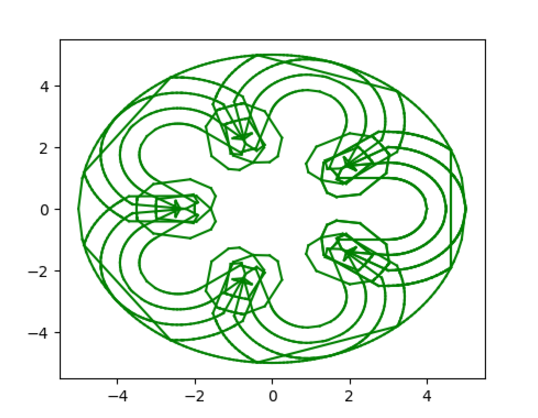
\includegraphics{testDemo}
    \caption{2D Modell med rotasjons feil}
    \label{fig:my_label}
\end{figure}
\noindent
Dette ble ikke plukket opp under testingen av funksjonen, men kom frem under senere testing.\\ \\
\noindent
Vi opplevde at testingen vår fungerte bra, da det bare var et vesentlig problem som ikke ble fanget opp. På tross av dette bør vi ha bedre retningslinjer for dette i fremtidige prosjekter, da vår fremgangsmåte er avhengig av at utviklerne er disiplinerte og lager gode tester på eget initiativ.\\ \\
\clearpage
\begin{figure}[h]

\lstset{language=Python, breaklines=true,} 
\begin{lstlisting}[frame=single]
def circleCrossing(line, r):
    p1 = line[0]
    p2 = line[1]
    #x^2*|p1|^2 + (x^2-2x+1)*|p2|^2 + 2x(1-x)*p1*p2 = R^2
    #(x^2-2x+1)*|p2|^2 = x^2*|p2|^2 - 2x*|p2|^2 + |p2|^2
    #2x(1-x)*p1*p2 = 2x*p1*p2 - 2x^2*p1*p2
    #x^2*p1^2 + x^2*p2^2 - 2x*p2^2 + p2^2 + 2x*p1*p2 - 2x^2*p1*p2 -R^2 = 0
    # = x^2*|p1|^2 + x^2*|p2|^2 - 2x^2*p1*p2 -2x*|p2|^2 + 2x*p1*p2 + |p2|^2 - R^2
    
    dotP1 = abs(p1[0]*p1[0] + p1[1]*p1[1])
    dotP2 = abs(p2[0]*p2[0] + p2[1]*p2[1])
    dotP1P2 = p1[0]*p2[0] + p1[1]*p2[1]
    #x^2*|p1|^2 + x^2*|p2|^2 - 2x^2*p1*p2
    a = dotP1 + dotP2 - 2*dotP1P2
    #-2x*|p2|^2 + 2x*p1*p2
    b = -2*dotP2 + 2*dotP1P2
    #|p2|^2 - R^2
    c = dotP2 - pow(r,2)
    
    #x = (-b+-sqrt(b^2-4ac) / 2a
    alpha1 = (-b + np.sqrt(pow(b,2)-4*a*c)) / (2*a)
    alpha2 = (-b - np.sqrt(pow(b,2)-4*a*c)) / (2*a)
    print "alpha1: ", alpha1
    print "alpha2: ", alpha2
    if -1 <= alpha1 <= 1:
        return alpha1
    else:
        return alpha2

a = [1,0]
b = [1,2]
line = [a, b]
x = circleCrossing(line, 2)
#x*p1 + (1-x)*p2
crossing = [x*a[0] + (1-x)*b[0],
            x*a[1] + (1-x)*b[1]]
print crossing
\end{lstlisting}
\caption{Test funksjon}
\end{figure}
\noindent
Isolert testing av funksjon for å finne kryssningen mellom en sirkel og et linjestykke, gitt linjestykket og radiusen til en sirkel sentrert i origo.
